\chapter{Logic-based Function Extraction}
\label{chap:integreat}

In the approaches to emulation-based measurements of system security we have considered thus far, the primary limitation has been the representation of missing information.
In real-world systems, components are often only partially accessible due to a mixture of closed-source code, limited physical accessibility, or intractable complexity.
Traditionally, the extraction of clean mathematical models from systems, such as ordinary differential equations, is considered infeasible.
Simultaneously, a significant amount of work has now been performed on the verification of models with black-box components, such as DryVR~\cite{fan2017dryvr}.
Systems such as these treat the numerous parameters of a black-box component as a continuous trajectory.
In this chapter, we will discover why this treatment of systems as black-box components, similar to the emulation-based approaches we have considered thus far, is not sufficient for the verification of systems.
We will introduce the InteGreat system~\cite{bland2023integreat}, which adopt a lifting approach to verification that extracts high-level emulations of systems from binary firmware.
In the latter sections of this chaper, we will demonstrate how this approach can be used to identify differences between implemented machine code and published mathematical specifications.

\section{Introduction}

Verification of cyber-physical systems (CPS) is a challenging problem, often simplified by the treatment of complex implemented components as black-boxes.
When considering the system itself, mathematical expressions for these systems must often be translated into low-level languages (C, Ladder Logic, etc.) and compiled for use in a physical system.
The resulting binary code may also be symbol-stripped and lose information, e.g. the names of variables, present in the original control algorithm.
In many cases, however, because the system retains something of the high-level semantics, it should still be possible to recover the original high-level model intended for a verification system.
As an added benefit, by working directly with firmware, we could verify and analyze programs where no high-level specification has been written.

While tools such as Ghidra~\cite{eagle2020ghidra} are capable of lifting a binary to pseudo-C representations, these outputs cannot be translated into a more abstract representation of the program.
Adapting these existing tools to lift to a given higher-level representation also requires significant effort, as their internal representations are static and aimed primarily at capturing microarchitectural semantics.
However, if natural deduction could be applied to express the nature of the semantic patterns as they appear in the binary, then lifting to a particular abstract representation could be made modular and portable.
This presents two particular problems of extraction and incorporation: in the former case, the ability to derive an abstract semantic from machine code operations, and the ability to incorporate outside information into the lifting process.

The current state of the art in function extraction involves the use of binary symbolic execution to derive a model of the binary's code over the theory of bitvectors, as was performed in part in Section~\ref{sec:jetset-eval}.
This approach deduces a mathematical model of a computation's behavior, but does not provide any framework for encoding common rules of abstraction.
Moreover, no current binary symbolic execution systems do not provide any means of precisely defining slices of the program to serve as boundaries for the lifting process, and rely on the user to isolate and substitute any subtrees of the AST for simplified expressions.
The result is a set of systems that could theoretically serve to automatically lift a binary to a higher-level representation based upon logical rules, but which in practice lack much of the necessary automation.

We therefore introduce InteGreat, a system which takes in a set of logical lifting rules (provided via Z3~\cite{zthree}) and outputs of symbolic execution to translate closed-source, symbol stripped binary firmware into verifiable mathematical models.
We achieve this by allowing users to nest and chain rules for lifting and decompilation in a natural, declarative syntax, allowing for the modular capture of complex semantic operations.
For example, we may associate a sequences of calls to multiple different child functions as a single operation and we lift a sequence of non-adjacent low level instructions into a single function call using the same effective syntax.
To our knowledge, this is the first lifter to use explicit logical propositions in targeting the correct abstract domain representation of a binary program.

InteGreat significantly extends the angr~\cite{angrsok} symbolic executor to bind the semantics of analyzed program slices into meaningful abstract symbols, replacing complex inner computations with a uniform representations, while maintaining the integrity of the symbolic state's semantics.
In particular, we focus on lifting to continuous equations that may be ``dropped in'' as Matlab Simulink function blocks~\cite{matlab} for evaluation in the context of an environmental model.
Under the system's default operation, a user only needs to specify entry and exit points in the firmware binary, and the system will replace function calls with uninterpreted functions, lifting sequences of otherwise complex operations into a single symbolic value.

To demonstrate the capabilities of such a system, we use InteGreat to show how logical rules can be used to lift continuous equations from a quad-copter firmware implementing Sebastian Madgwick's Orientation Filter~\cite{madgwick, drone}, and demonstrate these lifted equations uncover an implementation error in the quad-copter firmware, finding a three-way difference between the stabilization algorithm's mathematical representation, C, and third-party C implementations.
We also analyze a PLC firmware regulating a chemical plant's reactor pressure~\cite{ICSREF} and use the equations recovered by InteGreat to determine the sensor inputs necessary to precisely destabilize the reactor pressure of the chemical plant and exactly reproduce a code upload attack performed by prior literature.
The lifted representation of the chemical plant's firmware also communicates a subtle discovery: it is not possible to automatically infer representations of analog-to-digital unit conversions at I/O boundaries without additional information from a model of the physical environment.

\section{Related Work on Lifting}

This work brings together multiple methods from a rich history of verification of software and firmware systems.
While our discovery, the application of logics to the domain of decompilation and lifting, is novel, we are indebted to prior work for the introduction of nested abstractions, abstract interpretation, program slicing, function summarization, and many other techniques:

\begin{itemize}
	\item Currie et al.~\cite{currie2006embedded} use the substitution of program slices with uninterpreted functions to determine program equivalence across compiler optimizations.
	However, they do not address the idea of using nested logical rules to perform lift binary programs or the complexities involved in stitching together abstracted program slices.
	We provide a total framework for retaining viable semantics before and after skipping a program slice, even at the bitvector level.
	In fact, Currie et al. note that there may be ways to improve the accuracy of their matching by ``combining uninterpreted functions with a bit of bit-level analysis.''
	\item Sery et. al~\cite{interpolation} leverage the FunFrog system~\cite{sery2012funfrog} to extract function summaries after an initial verification run using source-code level symbolic execution to recover a Bounded Model Checker (BMC) logical formula representing the original program.
	The work performs AST slicing and variable binding methods similar to our own and uses the Craig interpolation (the identification of a sub-proposition that implies two other statements) to refine their function summaries.
	In contrast, InteGreat targets firmware and thus supports the abstraction of micro-architectural semantics.
	We also introduce the idea of using logical formulae to give rules for the translation rather than strict substitution of abstracted program slices based upon the semantics of the slices themselves (interpolation).
	\item A line of work has been done using symbolic execution to perform model extraction and subsequently verification on the extracted models.
	SPIN~\cite{spin}, defined the term ``model extraction'' and applied model-checking on aero-space flight software.
	Babi\'c and Hu~\cite{babic2007structural} used natural abstraction boundary identification and symbolic execution to optimize the performance of verification.
	Hernandez et al.~\cite{firmusb} and~\cite{cryto-symex} used symbolic execution to extract and verify protocol models.
	The same authors also noted the importance of rounding the floating-point precision error on verifying their extracted models in~\cite{precision}.
	Jackson and Woodward~\cite{lightweight-oo} extracted object-oriented (OO) models from Java byte-code,~\cite{oo-model} extracted OO data models from weakly-typed source code. 
	Bandera~\cite{tool-supported-program-abstraction} is a tool for user-guided extraction of finite-state automata from Java programs, however, the tool requires access to source code, and focuses on abstracting single variables rather than program slices.
	While all of these techniques could improve InteGreat, prior work does not address the possibility of a generic framework for the specification of lifting operations, and does not solve the specific problems involved in stitching together uninterpreted functions as abstractions.
	Our work also does not rely on static matching of semantic patterns and supports nested and chained natural deduction rules for lifting.
	\item Ji et al.~\cite{transformation} perform backward application of extended sequent calculus rules on symbolic expression trees.
	Our use of nested logical statements is similar to sequent calculus, however, the goal of Ji et al. was the bisimulation and optimization of the analyzed algorithms using sequent calculus, not to perform lifting.
\end{itemize}

Ultimately, we were somewhat suprised by the lack of a work approaching the subject of extracting functions from a system using logical operations.
However, this use case was also motivated by the specific insights introduced in the emulation and modeling of highly complex systems (Chapters~\ref{chap:rehost} and~\ref{chap:info}).
The InteGreat system draws on the specific challenges of the Jetset and Edact-Ray systems to inform its unique approach to the modeling of systems.

\section{Design of a Logic-based Lifting Specification}

We begin our design of InteGreat with program slices, introduced in Section~\ref{ref:lifting-prelim}, which we denote with $\gamma$, and the location of which we denote $f$.
By default we resolve each $\gamma$ to a function call boundary, but the determination of each $\gamma$'s location is also user-scriptable via a provided wrapper around Ghidra's static analysis APIs.
We enforce that the control flow of each slice must have either a total or no overlap with any other slice (an independence system).

As InteGreat runs, it begins analysis at the innermost $\gamma$ and works outward, identifying all the input and output locations (side effects) of each $\gamma$ via symbolic execution.
By default, these side effects are used to abstract the semantics of each $\gamma$ into a single uninterpreted function mapped to $f$ (the location of the call).
Specifically, we perform three actions upon reaching a location $f$ for a given $\gamma$:
\begin{enumerate}
	\item We associate $f$ to a set of logical formulae for lifting rules
	$\phi$, potentially input by a user, providing a deductive
	sepecification for \emph{how} to lift $f$. For example, encoding the
	logic of splitting a floating point value across r0 and r1.
	\item We associate $f$'s symbolic state with the set of input locations
	of $\gamma$: every potential register and memory location used by the
	output constraints provided by a full symbolic execution of $\gamma$.
	These are then available as symbols in $\phi$ to determine the
	appropriate parameterization of $f$.
	\item We associate encountering $f$ with a specific timestamp to ensure
	the lifted representation respects the program's order of operations.
\end{enumerate}

Our framework provides prospective solutions to the problems of unconstrained pointer values and loop invariant inference during symbolic execution.
To cope with unconstrained pointers we represent each read or write to memory with both the value and the symbolic expression used to determine the address, and enforce a strict equivalence between the two (discussed next).
We expect a zero-length program slice and associated $\phi$ to be defined which can be used to resolve any runtime-ambiguous values of pointers.
For many problematic loops, we can define two program slices: an outer which captures the formulae for handling the loop guard condition and an inner which captures the loop's body expression.
If suitable, we may then replace the guard condition with a concise symbolic represenation, e.g. $\Sigma$, and the inner with an inferred representation of the effects of the loop body as it relates to the outer operation.

As a fallback for fully automatic use of InteGreat, we accept the traditional symbolic execution search strategy of unrolling loops and provide a few sensible defaults for the search strategy, e.g. taking the state that generates the most complex set of constraints or the largest number of writes to memory.

Once the specific challenges of potential state explosion are dealt with, each $\gamma$ is associated to a new symbol $s_{0}, s_{1}, \dots$ and $\phi_{0}, \phi_{1}, \dots$ to perform a translation into a new, higher-level language.
These formulas are also \emph{nestable}, and rules may be written which take some $s$ and $\phi$ as input to produce a second $s'$ and $\phi'$.
For InteGreat's evaluation, we introduce $\phi$ and $\gamma$ such that unmanagable machine code is be abstracted into a Matlab-identical representation inside Z3.
Thus, theorem prover expressions serve as a flexible intermediate representation throughout the lifting process.

\paragraph{Symbolic Memory}
\label{sec:symb-mem-expl}
In most firmware programs, inputs and outputs are context-sensitive to its program state, for example, the dynamic execution stack, or a dereferenced pointer to a memory location.
It is thus necessary for InteGreat to allow symbolic expressions as memory addresses via a $LOC$ function.

InteGreat accomplishes this by implementing a symbolic memory model, extending Trt{\'\i}k et al.'s model~\cite{symbolic-memory}, under-constrained memory~\cite{Under-Constrained}, and incorporating the core ideas of Coppa et al.~\cite{coppa2017rethinking}.
Leveraging the angr event hook infrastructure, InteGreat intercepts all program state modifications, and replaces them with InteGreat's symbolic memory model. 
During each pointer dereference, the symbolic memory model is queried with the intercepted dynamic symbolic state of the symbolic executor.

We implement pointer reasoning by proving the equivalence of symbolic expressions for pointer values.
When resolving memory, we use timestamps associated with each memory operation and a strict equivalence check on the pointer expression to determine when a memory location is modified.
For example, given two pointers $p_{1}$ and $p_{2}$, if $p_{1} = 50$ and $p_{2} = 50$ at runtime and we are checking $read(p_{1}) = write(p_{2})$, we will return that they are NOT the same memory location. 
That is, we do not assume runtime knowledge. 
We assume that if such knowledge is needed, a zero-size program slice (an entry point address equivalent to the exit address) will be defined that will identify this runtime equivalence, and other tools exist for this~\cite{hind2001pointer}.

\paragraph{Correctness}
Traditional views of compiler (and by extension, decompiler) correctness involve ensuring uncompiled programs, interpreted over an input, result in the same output as compiled programs interpreted over the same input.
In the bottom-down view of compilation from a language operating over $\mathbb{R}$, we already implicitly accept the imprecision introduced by compiler/ISA when equations were compiled are executed.
One argument for the correctness of InteGreat's approach is that we may implicitly accept the imprecision introduced by the inverse operation: lifting from the ISA to the real domain semantics.

However, this does not deal explicitly with the information lost in InteGreat's approach to lifting, as features from the initial domain $\mathbb{D}$ may not be present in $\mathbb{D}'$.
In our earlier example, we mapped from an operation over a Galois field of 64-bit floating point values to an uninterpreted function over $\mathbb{R}$, and the semantics of the Galois field are not preserved in the uninterpreted function.
This trust in the decompiler is further strained when we begin to talk about abstracting arbitrary, complex program slices.
For example, the compiled version of a derivative function may be entirely different in implementation than a Matlab continuous domain equivalent.

We therefore rediscover a common solution to the problem of determining equivalence between complex computations: correctness is ensured by a reduction proof from the original function to the abstract function given a configurable error bound on the difference between outputs in $\mathbb{D}$ and $\mathbb{D}'$, $\varepsilon$.
A similar approach was outlined in Section~\ref{sec:encdec}.
The structure and representation of this proof is flexible and domain-specific, so long as it incorporates $\Phi$ and guarantees the limit $\varepsilon$ holds.
Proofs must be performed on a case-by-case basis as the non-abstracted function and targeted domains can take any of infinite forms.
For example, a proof for a straight-line program performing floating point operations could consider the error introduced by each operational step in the concrete case, and then chain these values together in order to derive a total acceptable bound for $\varepsilon$.
In the present chapter, we forgo a general proof and demonstrate equivalence empirically.

\paragraph{InteGreat's Interface}

\emph{Sufficient input to InteGreat is a program binary, an entry point at which to begin symbolic execution and a list of start and end addresses of program slices.} 
Slices $\gamma$ take the form of a range of addresses (potentially of zero length), a type of instruction, or an expression over the names of other slices.
To avoid repeating the same $\phi$ for multiple $\gamma$ referring to the same operations, we allow multiple range specifications for a given slice.
This input is provided by a series of files which name each $\gamma$ and provide $\Phi$ via a \emph{binds} array of assignments where the left hand side is a symbol name and the right hand side is a Z3 expression.

\emph{Binds} is initialized with the following two symbolic name sets:
\begin{enumerate}
	\item The inferred inputs of $\gamma$, e.g. i0, i1, \dots,
	\item Any prior expressions in the symbolic executor's state prior to reaching $\gamma$, and (optionally)
	\item The full \emph{inner} expression sets for $\gamma'$ inside of $\gamma$ before and after the application of the $\phi'$ associated to the specification of $\gamma'$.
\end{enumerate}
(3) is equivalent to preserving in memory the outputs of prior InteGreat lifting steps, allowing us to nest lifting rules in a modular fashion, and (2) allows us to ``chain'' lifting rules such that, given $\gamma'$ following $\gamma$, symbols returned by $\gamma$ can be used to reason about the lifting of returned by $\gamma'$.

The output of InteGreat is a simplified Z3 AST corresponding to the application of the lifting rules. 
In the evaluation of InteGreat, we structured program slices and inference rules such that translating the Z3 AST to Matlab was trivial.
However, the generic structure of Z3 as an intermediate representation makes it suitable for other tasks, e.g. inferring fixed points and loop invariants for lifted code~\cite{si2018learning}.

% All functions are implemented in Python 3.9.

% 2. \emph{Sequent Inference Algorithm} - This algorithm is used to perform sequent inference on the symbolic execution state.
% 3. \emph{Abstraction Resolution Algorithm} - This algorithm is used to perform abstraction resolution on the sequent inference results.
% 4. \emph{Director Algorithm} - This algorithm is used to perform symbolic execution on the merged state.

% Hooks & symbolic memory

\renewcommand{\algorithmicrequire}{\textbf{Input:}}
\renewcommand{\algorithmicensure}{\textbf{Output:}}

\begin{algorithm}
    \caption{Abstraction Lifting}
    \begin{algorithmic}[1]
        \Require $\gamma$, $binds$
        \Ensure $A_{\Phi(P)}^{f}$
	    \State $A_{P}^{f} \leftarrow SE_{\mathbb{D}}(\gamma)$
 	    \For{\textbf{each} i \textbf{in} inputs($A_{P}^{f}$)} \algorithmiccomment{Bind input to expressions}
	    \State $binds_{i} \leftarrow READ(LOC(i))$
        \EndFor
        \For{\textbf{each} o \textbf{in} outputs($A_{P}^{f}$)} \algorithmiccomment{Bind abstract expressions to output}
	
	    \State $E[outputs_{o}] \leftarrow \Phi_{\gamma}(o)$ \algorithmiccomment{Apply deduction rules}
	    \State $v \leftarrow new\_sym\_name()$
	    \State $binds_{v} \leftarrow E[outputs_{o}]$ \algorithmiccomment{Associate name to expression}
	    \State $WRITE(LOC(o), v)$ \algorithmiccomment{Write abstraction to symbolic memory}
        \EndFor

        \For{\textbf{each} b \textbf{in} $binds$}
	    \State $binds_{b} \leftarrow \Phi(b)$\algorithmiccomment{Common axiom support}
        \EndFor
    \end{algorithmic}
    \label{alg:abst-binding}
\end{algorithm}

\paragraph{InteGreat's Algorithm for Lifting}
\label{sec:integreat-alg}
Before describing the InteGreat's lifting algorithm, we introduce some notation.
Let $A_{P}^{f}$ to refer to the AST returned by angr prior to the application of $\Phi$, similar to Def.~\ref{def:nested-summarization}, and $E$ to refer to an intermediate storage location for Z3 AST expressions.
$\Phi_{\gamma}$ refers to the set of logical statements registered for $\gamma$, $\Phi_{\gamma}(o)$ refers to the full set of statements used to derive $o$ in $\Phi$ from the \emph{binds} array.
Recall that we also implement a symbolic memory addressing system for unconstrained pointer values; we represent locations (either in registers or memory) through the $LOC$ function.
Note that $READ$ and $WRITE$ operate on $A_{P}^{f}$ to produce $A_{\Phi(P)}^{f}$.
$SE_{\mathbb{D}}(\gamma)$ refers to an augmented form of symbolic execution of $\gamma$ using angr in the domain $\mathbb{D}$.

Algorithm~\ref{alg:abst-binding} presents InteGreat's core lifting mechanics.
As noted, the input to the algorithm is a program slice $\gamma$ and an existing set of symbolic bindings $binds$, and the output is a new AST $A_{\Phi(P)}^{f} \subseteq \mathbb{D}'$, representing the lifted program.
When $SE$ encounters an inner $\gamma'$, we look up the associated specification for $\gamma'$ and apply Alg.~\ref{alg:abst-binding} recursively to $\gamma'$ and propagate our results to the current symbolic state appropriately.

Line 1 retrieves a set of registers and memory locations $inputs, outputs$ describing the micro-architectural input and output locations of a program slice.
These are provided via a symbolic executor with modifications to support the use of symbolic values as memory addresses.
For locations with existing symbolic expressions, InteGreat's symbolic memory dynamically fetches the most recent written expression, or else InteGreat writes and returns a fresh symbolic variable in that location (the $READ$ function).

For values stored in memory, InteGreat dereferences the input locations to the correct symbolic expressions representing their values in InteGreat's symbolic memory model (discussed next).
These symbolic values are then assigned into the inputs symbols i0, i1, \dots of the \emph{binds} array (lines 2--4).
Note that the inputs may be sets of previously lifted abstractions.

InteGreat then replaces the existing lower-level, concrete expressions returned by symbolic execution for the slice's outputs with the higher-level abstraction (lines 5--10).
For example, consider a floating point multiply over registers $r_{0}$ and $r_{1}$, with output in $r_{0}$, with a simple $\phi$ that returns an uninterpreted function $f$ over the inputs.
A fresh symbolic variable $v$ would be created and written to the symbolic memory model, with the concrete register location $r_{0}$ storing $r_{0} = v \mapsto f(i_{0},i_{1})$ rather than $r_{0} = i_{0} * i_{1}$.
This step also introduces fresh symbolic mappings to expressiosn in the \emph{binds} state.
All future symbolic execution and calls to Alg.~\ref{alg:abst-binding} will now operate on the abstractions provided by $binds$ rather than the original concrete symbolic expression for $\gamma$.

Lines 11 through 13 of Alg.~\ref{alg:abst-binding} provide support for common axioms.
The full set of $\Phi$ for $\gamma$ are reapplied at the end of analysis to resolve existing AST features into higher-level abstractions.
We found this useful for lifting certain common operations across different slices.
For example, we created rules for treating certain type-casts as equivalent, e.g. when a double is rounded to a float or a float is extended to a double, the Galois field variable should still refer to the same lifted variable over $\mathbb{R}$.

\section{Experiments on a Quad-copter and Programmable Logic Controller}

This section presents the evaluation of InteGreat on a quad-copter firmware and a PLC firmware stabilizing the reactor pressure of a chemical plant.
% All experiments were conducted on an Intel 11th Gen 16 Core i7-11850H 2.50 GHz Processor with 16.0 GB of RAM.
In particular, we investigated a few concrete questions regarding the possiblities of InteGreat's design.
We first consider whether, given the correct $\Phi$, InteGreat can correctly lift machine code programs to the continuous domain.
Next, we determine whether InteGreat's approach can help identify inconsistencies between published results and different implementations of the same algorithm.
Then, InteGreat's lifted representations are testing in the analysis and discovery of novel features in a Progammable Logic Controller.
Finally, we consider whether it is possible to correctly reproduce idealized models and attacks on cyberphysical systems using InteGreat's lifted representations.

To answer these questions, we evaluate InteGreat on two real-world embedded systems: a quad-copter firmware and a PLC firmware.
We considered the firmware for both of these systems to be closed-source and symbol-stripped: the inputs to InteGreat are not dependent on any meaningful variable names or function names.
We also not that the firmware was not obfuscated, and that the firmware is not using any anti-analysis techniques.

\begin{figure*}
    \centering
    \hfill
	\begin{subfigure}[b]{0.49\textwidth}{}
	\centering
	\resizebox{0.8\width}{0.8\height}{
\begin{tikzpicture}[xscale=0.8, every node/.style={scale=0.80}]
  \def\t{0.01} % stem half-thickness
    \node[above] at (1, 0.3)(fmul) {fmul};
    \node[above] at (2, 0.3)(addsf3) {...};
    \node[above] at (3, 0.3)(f2d) {f2d};
    \node[above] at (4, 0.25)(sqrt) {sqrt};
    \node[above] at (5, 0.3)(truncdfsf) {trunc};
    \node[above] at (6, 0.3)(fsub) {...};
    \node[above] at (7, 0.3)(muldf3) {muldf};
    \node[above] at (8, 0.3)(divdf3) {divdf};
    \node[above] at (9, 0.3)(fdiv) {...};
    \node[above] at (10, 0.3)(atan2) {atan2};
    \node[above] at (11, 0.3)(asin) {asin};
    \node[above] at (12, 0.25)(fcmpeq) {fcmpeq};
  % BRANCHES
  \draw[branch,line width=4] (0,0) -- (13,0) ;
   % node[right] {Quadcopter};

    \draw[branch,thick] (fcmpeq) to (12, -0.3) node[below] {1.0};

  \draw[branch,thick] (fmul) to (1, 1.5);
  \draw[branch,thick] (5,1.3) -- (5,1.5);
  \draw[branch,thick] (1,1.5) -- (5,1.5) node[midway,above] {mul};

  \draw[branch,thick] (f2d) to (3, 1);
  \draw[branch,thick] (muldf3) to (7, 1);
  \draw[branch,thick] (truncdfsf) to (5, 1);
  \draw[branch,thick] (3,1) -- (7,1) node[midway,above] {cmul};

  \draw[branch,thick] (f2d) to (3, -0.3);
  \draw[branch,thick] (sqrt) to (4, -0.3);
  \draw[branch,thick] (truncdfsf) to (5, -0.3);
  \draw[branch,thick] (3,-0.3) -- (5,-0.3) node[midway,below] {csqrt};
  
  \draw[branch,thick] (3, -0.5) to (3, -0.8);
  \draw[branch,thick] (5, -0.5) to (5, -0.8);
  \draw[branch,thick] (muldf3)  to (7, -0.8);
  \draw[branch,thick] (divdf3)  to (8, -0.8);
  \draw[branch,thick] (atan2)  to (10, -0.8);
  \draw[branch,thick] (3, -0.8) -- (10, -0.8);
    \node[above] at (6, -0.8) {catan2};

  \draw[branch,thick] (3, -1) to (3, -1.3);
  \draw[branch,thick] (5, -1) to (5, -1.3);
  \draw[branch,thick] (7, -1)  to (7, -1.3);
  \draw[branch,thick] (8, -1)  to (8, -1.3);
  \draw[branch,thick] (asin)  to (11, -1.3);
  \draw[branch,thick] (3, -1.3) -- (11, -1.3) node[midway,below] {casin};


  \draw[branch,thick] (1, 0) to (fmul);
  \draw[branch,thick] (2, 0) to (addsf3);
  \draw[branch,thick] (3, 0) to (f2d);
  \draw[branch,thick] (4, 0) to (sqrt);
  \draw[branch,thick] (5, 0) to (truncdfsf);
  \draw[branch,thick] (6, 0) to (fsub);
  \draw[branch,thick] (7, 0) to (muldf3);
  \draw[branch,thick] (8, 0) to  (divdf3);
  \draw[branch,thick] (9, 0) to (fdiv);
  \draw[branch,thick] (10, 0) to  (atan2);
  \draw[branch,thick] (11, 0) to (asin);
  \draw[branch,thick] (12, 0) to (fcmpeq);
  
\end{tikzpicture}
}
\caption{}
\end{subfigure}
\hfill
\begin{subfigure}[b]{0.49\textwidth}
\centering
\begin{tabular}{ |l|ccc| } 
 \hline
  Version & \#Lifts & \#Symbols & \#LoA \\ [0.5ex] 
 \hline
 \hline
  Firmware & 335 & 151 & 728 \\ [0.3ex] 
  Corrected & 343 & 149 & 730 \\ [0.3ex] 
  Published & 283 & 159 & 637 \\ [0.3ex] 
 \hline
\end{tabular}
	\caption{}
\label{fig:table-madgwick}
\end{subfigure}
\hfill
\caption{\textbf{(a)}: Depiction of hierarchy of lifting rules for a quad-copter stabilization algorithm. \textbf{(b)}: Quad-copter firmware analytics, broken down into the number of program slice locations lifted, unique symbolic variables used, and lines of assembly code (LoA).}
\label{fig:quad-analytics}
\end{figure*}



The quad-copter firmware was compiled for ARM32, EABI5 version 1, and statically linked.
We targeted four versions of the quad-copter's stabilization algorithm, a compiled version present in a firmware image on Github~\cite{drone}, a version compiled from the specification given by the algorithm's original publication~\cite{madgwick}, a \emph{correct} version of the algorithm written for Matlab, and a \emph{correct} version of the algorithm written in C, compiled using the same ARM compiler, and then lifted by InteGreat.

\begin{table}
\caption{14 of the 18 quad-copter \emph{binds} array elements used to lift continuous equations from binary firmware using InteGreat.}
\label{tab:quadcopt-binds}
\begin{tabular}{|l|p{11cm}|}
	\hline
	\textbf{Program slice C code name} & \textbf{Associated \emph{binds} array} \\ \hline
	\hline
\_\_addsf3       & 

"o0": "binds['i0'] + binds['i1']"
 \\ \hline
\_\_aeabi\_f2d    & 

"tmp": "z3.fpToFP(z3.RNE(), binds['i0'], z3.FPSort(11, 53))",
 \\
                      & 

"o0": "z3.Extract(31, 0, z3.fpToIEEEBV(binds['tmp']))",
 \\
                      & 

"o1": "z3.Extract(63, 32, z3.fpToIEEEBV(binds['tmp']))"
 \\ \hline
\_\_aeabi\_fcmpeq & 

"o0": "z3.If(binds['i0'] == binds['i1'], z3.FPVal(1.0, z3.FPSort(8, 24)), z3.FPVal(0.0, z3.FPSort(8, 24)))"
 \\ \hline
\_\_aeabi\_fdiv & 

"o0": "binds['i0'] / binds['i1']"
 \\ \hline
\_\_aeabi\_fmul & 

"o0": "binds['i0'] * binds['i1']"
 \\ \hline
\_\_aeabi\_fsub & 

"o0": "binds['i0'] - binds['i1']"
 \\ \hline
\_\_divdf3 & 

"tmp": "z3.fpBVToFP(z3.Concat(binds['i1'], binds['i0']), z3.FPSort(11, 53)) / z3.fpBVToFP(z3.Concat(binds['i3'], binds['i2']), z3.FPSort(11, 53))",
 \\
                      & 

"o0": "z3.Extract(31, 0, z3.fpToIEEEBV(binds['tmp']))",
 \\
                      & 

"o1": "z3.Extract(63, 32, z3.fpToIEEEBV(binds['tmp']))"
 \\ \hline
\_\_muldf3 & 

"tmp": "z3.fpBVToFP(z3.Concat(binds['i1'], binds['i0']), z3.FPSort(11, 53)) * z3.fpBVToFP(z3.Concat(binds['i3'], binds['i2']), z3.FPSort(11, 53))",
 \\
                      & 

"o0": "z3.Extract(31, 0, z3.fpToIEEEBV(binds['tmp']))",
 \\
                      & 

"o1": "z3.Extract(63, 32, z3.fpToIEEEBV(binds['tmp']))"
 \\ \hline
\_\_truncdfsf2 & 

"o0": "z3.fpToFP(z3.RNE(), z3.fpBVToFP(z3.Concat(binds['i1'], binds['i0']), z3.FPSort(11, 53)), z3.FPSort(8, 24))"
 \\ \hline
asin & 

"tmp": "z3.Function('asin', *[z3.BitVecSort(32) for \_ in range(2)], z3.BitVecSort(64))(binds['i0'], binds['i1'])",
 \\
                      & 

"o0": "z3.Extract(31, 0, binds['tmp'])",
 \\
                      & 

"o1": "z3.Extract(63, 32, binds['tmp'])"
 \\ \hline
atan2 & 

"o0": "z3.Extract(31, 0, z3.Function('atan2', *[z3.BitVecSort(32) for \_ in range(4)], z3.BitVecSort(64))(binds['i0'], binds['i1'], binds['i2'], binds['i3']))",
 \\
                      & 

"o1": "z3.Extract(63, 32, z3.Function('atan2', *[z3.BitVecSort(32) for \_ in range(4)], z3.BitVecSort(64))(binds['i0'], binds['i1'], binds['i2'], binds['i3']))"
 \\ \hline
sqrt & 

"tmp": "z3.fpSqrt(z3.RNE(), z3.fpBVToFP(z3.Concat(binds['i1'], binds['i0']), z3.FPSort(11, 53)))",
 \\
                      & 

"o0": "z3.Extract(31, 0, z3.fpToIEEEBV(binds['tmp']))",
 \\
                      & 

"o1": "z3.Extract(63, 32, z3.fpToIEEEBV(binds['tmp']))"
 \\ \hline
neg & 

"o0": "-binds['i0']"
 \\ \hline
csqrt & 

"o0": "z3.Function('csqrt', z3.FPSort(8, 24), z3.FPSort(8, 24))(binds['\_\_aeabi\_f2d']['i0'])"
 \\ \hline
% cfcmpeq & 
% 
% "o0": "z3.FPVal(0.0, z3.FPSort(8, 24))"
%  \\ \hline
% cmul & 
% 
% "o0": "z3.fpToFP(z3.RNE(), z3.fpToFP(z3.RNE(), binds['\_\_aeabi\_f2d']['i0'], z3.FPSort(11, 53)) * z3.fpBVToFP(z3.Concat(binds['\_\_muldf3']['i3'], binds['\_\_muldf3']['i2']), z3.FPSort(11, 53)), z3.FPSort(8, 24))"
%  \\ \hline
% casin & 
% 
% "o0": "z3.fpToFP(z3.RNE(), z3.fpToFP(z3.RNE(), z3.Function('asin', z3.FPSort(8, 24), z3.FPSort(8, 24))(binds['\_\_aeabi\_f2d']['i0']), z3.FPSort(11, 53)) * z3.fpBVToFP(z3.Concat( binds['\_\_muldf3']['i3'], z3.BitVecVal(0, 32)), z3.FPSort(11, 53)) / z3.fpBVToFP(z3.Concat(binds['\_\_divdf3']['i3'], binds['\_\_divdf3']['i2']), z3.FPSort(11, 53)), z3.FPSort(8, 24))"
%  \\ \hline
% catan2 & 
% 
% "o0": "lambda binds: z3.fpToFP(z3.RNE(), z3.fpToFP(z3.RNE(), z3.Function('catan2', z3.FPSort(8, 24), z3.BitVecSort(32), z3.FPSort(8, 24))(binds['\_\_aeabi\_f2d']['i0'], binds['atan2']['i2']), z3.FPSort(11, 53)) * z3.fpBVToFP(z3.Concat(binds['\_\_muldf3']['i3'], z3.BitVecVal(0, 32)), z3.FPSort(11, 53)) / z3.fpBVToFP(z3.Concat(binds['\_\_divdf3']['i3'], binds['\_\_divdf3']['i2']), z3.FPSort(11, 53)), z3.FPSort(8, 24))"
%  \\
%  \hline
\end{tabular}

\end{table}

The inputs to InteGreat used to lift the quad-copter firmware consisted of 18 program slices ($\gamma$) and 24 \emph{binds} entries ($\Phi$). %, given in Appendix Table~\ref{tab:quadcopt-binds}
We depict the results of these lifting rules in Fig.~\ref{fig:quad-analytics}, and include the specification of 16 these bindings in Table~\ref{tab:quadcopt-binds} as an example.
The left side demonstrates the structure by which we were able to nest lifting rules.
The right side demonstrates the modularity of lifting rule applications across different code locations, i.e. the slice for lifting a floating point multiply could be applied across several distinct code locations.


\begin{figure}
    \centering
%     \hfill
% \begin{subfigure}[b]{0.49\textwidth}{}
% \centering
% \resizebox{1\width}{1\height}{%
% \begin{tikzpicture}[xscale=0.65, every node/.style={scale=0.80}]
%   \def\t{0.01}
%     \node[above] at (3, 0.3)(integ0) {integral\_0};
%     \node[above] at (6, 0.3)(deriv0) {derivative\_0};
%     \node[above] at (9, 0.3)(integ1) {integral\_1};
%     \node[above] at (12, 0.3)(deriv1) {derivative\_1};
% 
%   \draw[branch,thick] (integ0) to (3, 1);
%   \draw[branch,thick] (6,1) -- (deriv0);
%   \draw[branch,thick] (3,1) -- (6,1) node[midway,above] (plrprg0) {PID\_0};
% 
%   \draw[branch,thick] (integ1) to (9, 1);
%   \draw[branch,thick] (12,1) -- (deriv1);
%   \draw[branch,thick] (9,1) -- (12,1) node[midway,above] (plrprg1) {PID\_1};
% 
%   \draw[branch,thick] (plrprg0) to (4.5, 1.6);
%   \draw[branch,thick] (10.5,1.6) -- (plrprg1);
%   \draw[branch,thick] (4.5,1.6) -- (10.5,1.6) node[midway,above] (pidfixcycle) {plc\_prg};
% \end{tikzpicture}
% 	}
% 	\label{fig:plc-abstr}
% \end{subfigure}
% \hfill
% \begin{subfigure}[b]{0.49\textwidth}
% \centering
\begin{tabular}{ |l|ccc| } 
 \hline
  Function & \#Lifts & \#Symbols & \#LoA \\ [1ex] 
 \hline
 \hline
  integral & 0 & 5 & 47 \\ [0.5ex] 
  derivative & 0 & 10 & 24 \\ [0.5ex] 
  pid & 8 & 9 & 302 \\ [0.5ex] 
  main & 2 & 6 & 148 \\ [0.5ex] 
 \hline
\end{tabular}
\label{fig:table-plc}
% \end{subfigure}
	\caption{Analytics for InteGreat's lifting of the PLC firmware's control logic. The integral and derivative functions contained no inner program slices. Each call to PID, integral, and derivative maintains separate state.}
% \hfill
	\label{fig:plc-stats}
\end{figure}



The PLC firmware was compiled both using CoDeSys 2.3.9.44 and e!COCKPIT 3.5.16.30 for the WAGO 750-881 and PFC200 G2 750-8217 PLCs, respectively.
We recovered the same results for both of these PLCs and present the results for the latter in this paper, as it is the more recent version.
Both PLCs use the same CPU architecture (ARM32), and the firmware is statically linked.

We targeted an algorithm in PLC firmware for actuating a pressure-controlling valve in the Tennessee Eastman Challenge~\cite{Tennessee-Eastman}, a benchmark for modeling and analyzing the dynamics of industrial control systems.
The firmware is written in the structured text, IEC 61131-3, programming language and then compiled to a binary for the PLC.
The firmware in question was provided by ICSREF~\cite{ICSREF}, a security paper which staged a code upload attack on a physical PLC connected to a Matlab environmental model.
Additional details of this attack's physical setup are given in~\cite{keliris2016machine}.

The specification used to lift the PLC firmware consisted of 3 program slices and 3 \emph{binds} entries generating uninterpreted functions for three cases: a proportional-integral-derivative call, a derivative call, and an integral call.
We depict the results of these lifting rules in Fig.~\ref{fig:plc-stats}.
The PLC had significantly fewer binds as it did not rely on a software floating point ABI and Matlab, the target domain, had pre-existing functions for integral and derivative.

\subsection{Correct Lifting of a Quad-Copter Stabilization Algorithm}

We evaluated InteGreat\ by recovering equations for continuous orientation estimation from an open-source, MCU-based quad-copter autopilot controller.
The firmware we studied implemented Madgwick's Gradient Descent Orientation Filter~\cite{madgwick}.
The orientation estimator takes in sensor inputs from the IMU consisting of an accelerometer, gyroscope, and magnetometer.
Orientation Estimators for strapdown INS (Inertial Navigation Systems) \emph{continuously} fuse sensor data with previous estimations and obtain new attitude across the time domain.
Because of this, difference in implementations that are subtle on the surface lead to large accumulative error across small time periods.

We ran four experiments using different versions of Madgwick's algorithm to showcase InteGreat's ability in detecting bugs and algorithm variants in firmware.
These experiments are depicted in Fig.~\ref{fig:madg}, through a simulation of the quad-copter spinning in three dimensions.
These simulations were performed using Matlab's ``rpy\_9axis'' sensor data.

\begin{figure*}
    \centering
    \begin{subfigure}[b]{0.327\textwidth}
        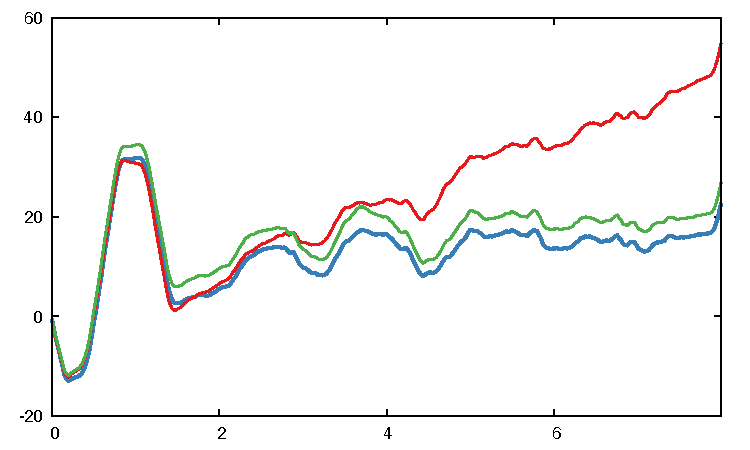
\includegraphics[width=\textwidth]{madg_data/pitch.pdf}
	    \caption{Pitch}
    \label{fig:pitch}
    \end{subfigure}
    \hfill
    \begin{subfigure}[b]{0.327\textwidth}
        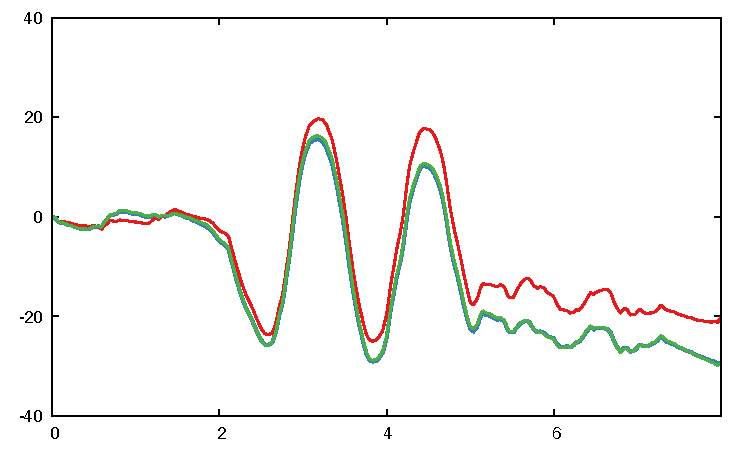
\includegraphics[width=\textwidth]{madg_data/yaw.pdf}
        \caption{Yaw}
        \label{fig:yaw}
    \end{subfigure}
    \hfill
    \begin{subfigure}[b]{0.327\textwidth}
        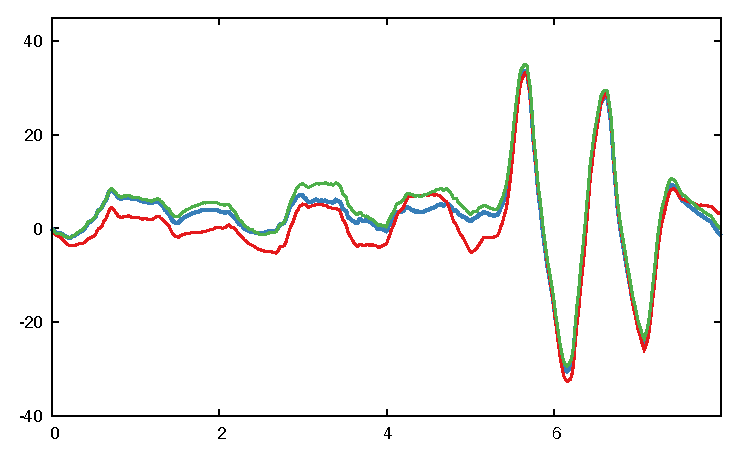
\includegraphics[width=\textwidth]{madg_data/roll.pdf}
        \caption{Roll}
        \label{fig:roll}
    \end{subfigure}
    \hfill
    \caption{Empirical results measuring the ability of InteGreat's recovered models of Orientation Estimation algorithms to identify bugs.}
    \label{fig:madg}
\end{figure*}

Note that only three lines are present in Fig.~\ref{fig:madg}.
The fourth line, the correct Matlab implementation, the blue line, is identical to lifted version of a corresponding correct C implementation.
This finding ensures InteGreat\ did not make mistakes while lifting, and was able to produce identically behaving Matlab code with respect to compiled C firmware code.
The equivalence between the two correct implementations gives us confidence in the methodology InteGreat\ introduces.

The figure depicts the same inputs to the IMU sensor of a device oscillating in pitch, yaw, then roll. \textbf{Green} is lifted by InteGreat\ from \emph{real world} firmware that contains a bug. \textbf{Blue} contains \emph{two} lines: the InteGreat\ lifted firmware recompiled to correct the gradient calculation, and \emph{a correct} Matlab implementation of Madgwick's algorithm. \textbf{Red}, however, is a compiled firmware using the \emph{faulty} C code included in Madgwick's published report. This version has accumulative error with respect to the earth's magnetic field.

Continuous equations lifted by InteGreat\ were identical to ground truth simulations in a controlled IMU sensor experiment rotating the quadcopter in 3 dimensions using 1,600 measurement points. This demonstrates our framework is able to lift correct continuous equations from discrete, machine code implementations and verify them using tools operating over the abstract domain.

\paragraph{Example of InteGreat Identifying Bugs}
\label{sec:quadcopter}

%Even the proposer of this algorithm published two variants, one C implementation in the appendix of his report and a Matlab implementation on his website after the Orientation Filter became increasingly popular for commodity drones ~\cite{}.

We next evaluate whether InteGreat\ is useful when attempting to identify bugs in firmware.
When comparing the Madgwick-provided Matlab implementation (blue) with the version recovered from the \emph{real world} firmware implementation (green), we discovered an error in the gradient of the solution surface which is calculated by multiplying the objective Function matrix and its Jacobian matrix: $\nabla F = \mathbf{J}^T(_{E}^{S}\hat{\mathbf{q}},^{E}\hat{\mathbf{b}}) \mathbf{F}(_{E}^{S}\hat{\mathbf{q}},^{E}\hat{\mathbf{b}}, ^{S}\hat{\mathbf{a}}, ^{S}\hat{\mathbf{m}})$.
Comparing the correct magnetic field components of the Objective Function with the InteGreat\ lifted version (using normalized magnetic field sensor values for simplicity):

\newcommand*{\Scale}[2][4]{\scalebox{#1}{$#2$}}%
$$
\mathbf{f}_b(_{E}^{S}\hat{\mathbf{q}},^{E}\hat{\mathbf{b}} ^{S}\hat{\mathbf{m}}) = 
\begin{bmatrix}
    2b_{x}(0.5-q_{3}^{2}-q_{4}^{2})+2b_{z}(q_{2}q_{4}-q_{1}q_{3})-m_{x}\\
    2b_{x}(q_{2}q_{3}-q_{1}q_{4})+2b_{z}(q_{1}q_{2}+q_{3}q_{4})-m_{y}\\
    2b_{x}(q_{1}q_{3}+q_{2}q_{4})+2b_{z}(0.5-q_{2}^{2}-q_{3}^{2})-m_{z}\\
\end{bmatrix}
$$

\[
\begin{aligned}
	F_4 &= ((0.5 + (- q_3 ^ 2 ) + (- q_4 ^ 2 ))  * b_x  + (q_2 * q_4  + (- q_1 * q_3 )) * b_z + (- m_x) \\
	F_5 &= (q_2 * q_3  + (- q_1 * q_4 )) * b_x + (q_3 * q_4 + q_1 * q_2) * b_z + (- m_y) \\
	F_6 &= (((0.5 + (- q_2 ^ 2)) + (- q_3 ^ 2))  * b_z  + (q_1 * q_3  + q_2 * q_4 ) * b_x + (- mz) \\
\end{aligned}
\]
\normalsize

It is clear that terms using the earth’s magnetic field ($^{E}\hat{\mathbf{b}}$) in the Objective Function have missing coefficients.\footnote{
	$b_{y}$ is not present as the earth’s magnetic field is be considered to have components in one horizontal axis and the vertical axis.}
The same errors occur in all magnetic field components of the Jacobian.
We compare only one row of the Jacobian here for simplicity:

\[
\begin{aligned}
    J_{4,1}&= (-q_3*b_z) \\
    J_{4,2}&= (q_4*b_z) \\
    J_{4,3}&= (q_3*(-2*b_x)+(-q_1*b_z)) \\
    J_{4,4}&= (q_4*(-2*b_x)+(q_2*b_z)) \\
\end{aligned}
\]
\[
\begin{aligned}
    \mathbf{J_4}(_{E}^{S}\hat{\mathbf{q}},^{E}\hat{\mathbf{b}}) &= \begin{bmatrix}
    -2b_zq_3, & 2b_zq_4, & -4b_xq_3-2b_zq_1,  & -4b_xq_4+2b_zq_2 \\
\end{bmatrix}\\
\end{aligned}
\]
\normalsize

%TODO: Is there something to be said about accumulated errors and how attacks can be made more stealthy?
After correcting all coefficients of the earth’s magnetic field ($^{E}\hat{\mathbf{b}}$) and recompiling the quad-copter firmware, the continuous equations lifted by InteGreat\ exactly matched Madgwick's Matlab implementation (blue).

We then compared the corrected equations (blue) with a \emph{third} firmware version, compiled to use Madgwick's published implementation, written in C, which is included in the original Madgwick paper (red).
We found that the published variant of the algorithm recursively feeds in previously calculated gyroscopic biases multiplied by a correction constant $\zeta$.
In contrast, existing implemented algorithms did \emph{not} perform gyroscopic bias removal and instead used dynamically calculated flux vectors of the Earth's frame in the equation's objective function.
This further confirmed InteGreat's ability to help researchers understand differences between implementations and published results.

% research question answer
By lifting compiled machine code to continuous equations using logical reasoning, it is possible to identify bugs in firmware implementations and check the validity of published results.
Validation can be performed by comparing representations which, after lifting, operate over the same domain, or by using a framework to check output equivalence, i.e. reachability, between algorithm versions.

% InteGreat's output was:
% $$
% \begin{aligned}
%     &w_{errz} = ((2 * q_1  * s_4) + (- 2 * q_2 * s_3)  + (2 * q_3 * s_2) + (- 2 * q_4 * s_1))\\
%     &w_{erry} = ((2 * q_1  * s_3)  + (2 * q_2 * s_4) + (- 2 * q_3 * s_1) + (- 2 * q_4 * s_2))\\
%     &w_{errx} = ((2 * q_1  * s_2)  + (- 2 * q_2 * s_1) + (- 2 * q_3 * s_4) + (2 * q_4 * s_3))\\
%     &w_{bz} = (w_{errz} * \zeta * \delta_t + w_{bz})\\
%     &w_{by} = (w_{erry} * \zeta * \delta_t + w_{bx})\\
%     &w_{bx} = (w_{errx} * \zeta * \delta_t + w_{by})\\
% \end{aligned}
% $$



% Taking in account the numerous different implementations of the Madgwick Orientation Filter, we consider a Madgwick Orientation Filter to be \emph{Correct} if the gradient calculation is the same as published in Madgwick's paper, and the gradient correctly updates the quaternion; \emph{Complete} if the Orientation estimation is within reasonable error range of the algorithm published by Madgwick.

% \begin{figure}
%     \centering
%     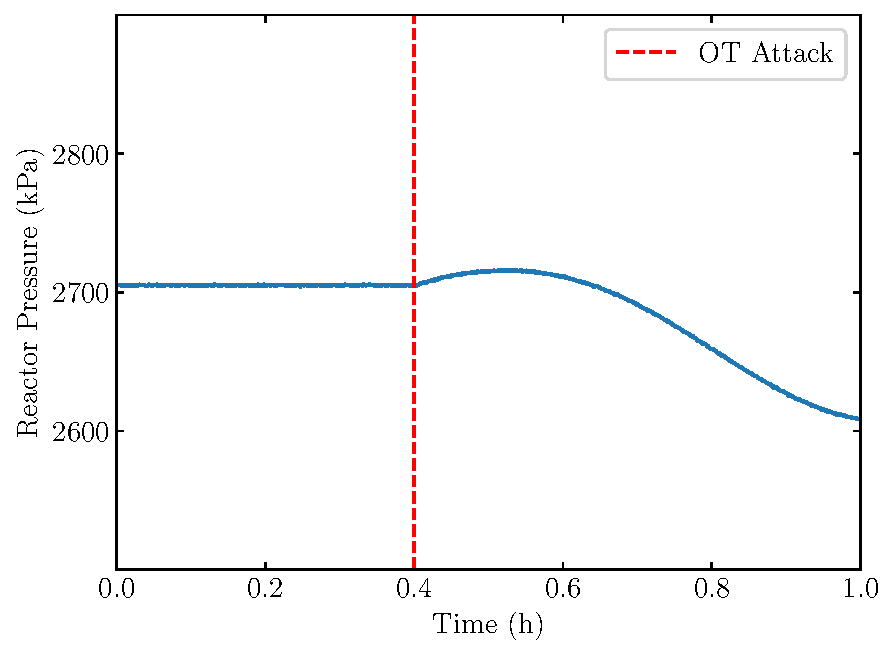
\includegraphics[width=0.4\textwidth]{plc_data/plot.pdf}
%     \caption{Simulated OT attack on the continuous equations \emph{lifted} from closed source, symbol-stripped PLC firmware.}
%     \label{fig:te_attack}
% \end{figure}





\subsection{Analyzing and Extracting Functions from PLC Firmware}
\label{sec:plc}

In this section, we demonstrate our ability to analyze continuous equation models of the firmware of a PLC (Fig.~\ref{fig:plc-stats}).
We recovered the following core model from the firmware's PID (proportional-integral-derivative) functions, where I and D are uninterpreted functions for integral and derivative, respectively:
\begin{equation}
v_{6}(
(v_{3}-v_{2})+
\frac{1}{v_{5}}
I(v_{3}-v_{2},1000t)
+
v_{1}
D(v_{3}-v_{2},1000t)
)+v_{0}+v_{7}
    \label{eqn:ideal_pid_fixcycle}
\end{equation}

For analysis in Matlab, we needed to also take into account some non-infinitesimal measure of time.
We simplified the recovered equation further via a few additional common axioms, e.g. $new\_sym = v_{3} - v_{2}$, $integ\_e\_dt = I(binds_{i0}, binds_{i1})$:
\begin{equation}
    K_{p}(
        e + 
        \frac{1}{\tau_{i}}
        \int e \mathrm{d}t
        + 
        \tau_{d}
        dv e t
    ) + b
    \label{eqn:ideal_pid_fixcycle}
\end{equation}

Eqn.~\ref{eqn:ideal_pid_fixcycle} more closely matches the traditional PID formulation, where $K_{p}$ is the proportional gain constant the ICSREF attack modified.
The other equations InteGreat\ recovered from the PLC did not require further constructed abstraction specifications.

\textbf{Discovering Additional Hardware.}
In the lifted version of the firmware, we also found an obscure scaling was applied to the sensor value for the input reactor pressure before it was supplied to Eqn.~\ref{eqn:ideal_pid_fixcycle}:

\begin{equation}
    P = 1000(((P_{digital} / 30000) - 0.0046) / 0.9876) + 2000
	\label{eqn:input-conv}
\end{equation}

\begin{figure*}
    \centering
    \begin{subfigure}[b]{0.49\textwidth}
        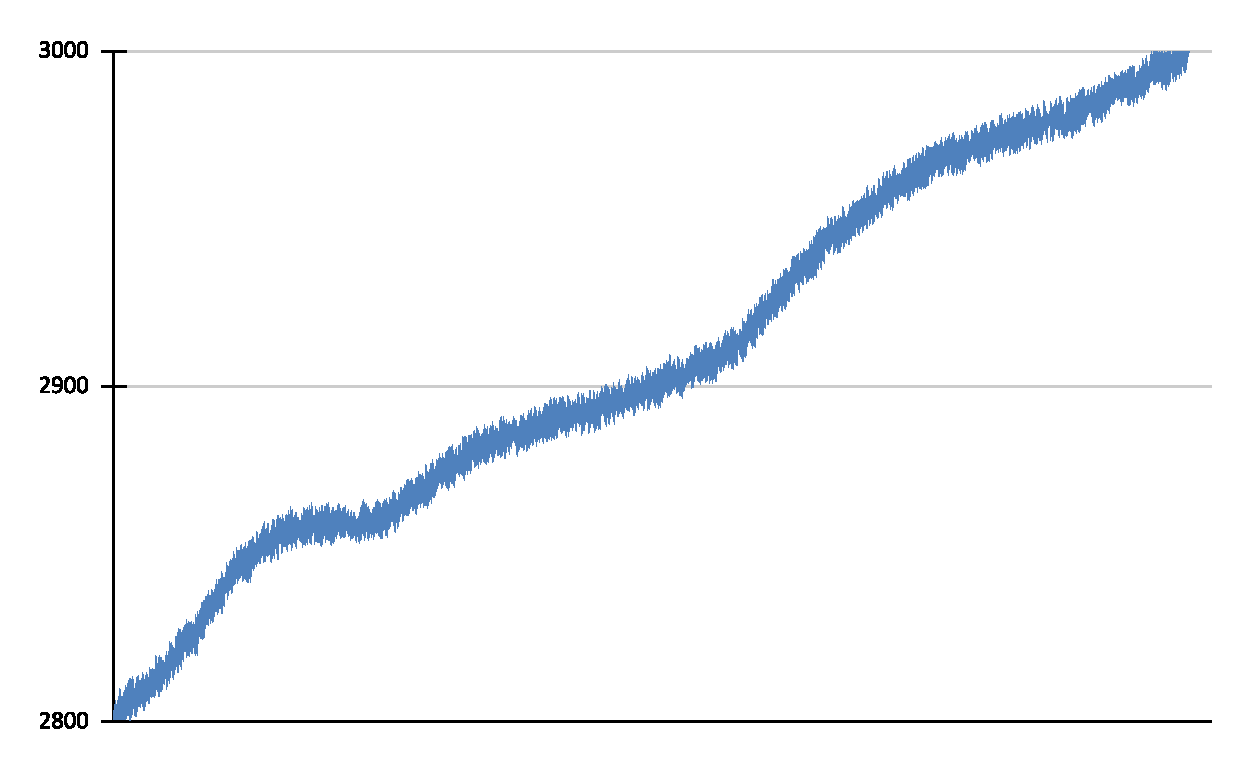
\includegraphics[width=\textwidth]{fig/plc-orig.pdf}
        \caption{Naive Attack Reproduction}
        \label{fig:orig-attack}
    \end{subfigure}
    \hfill
    \begin{subfigure}[b]{0.49\textwidth}
        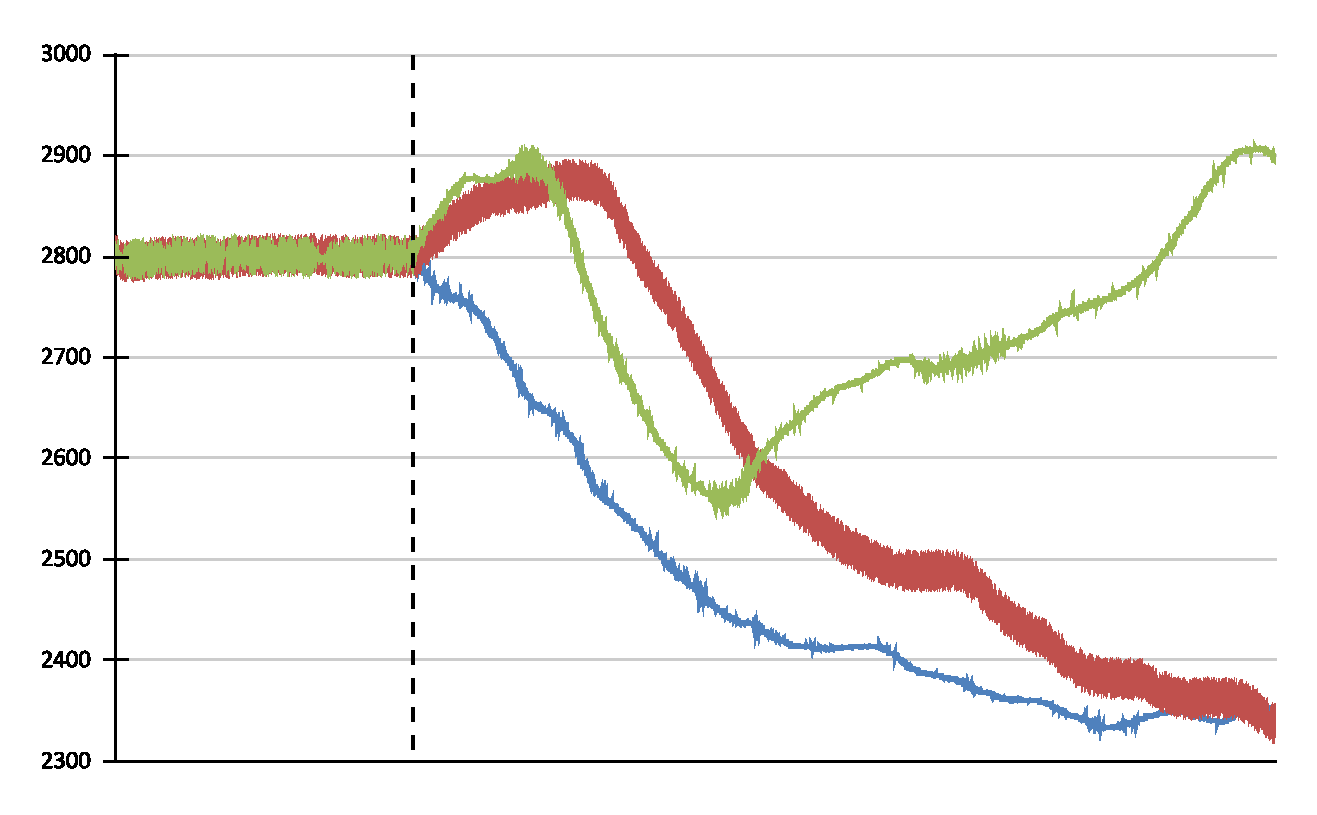
\includegraphics[width=\textwidth]{fig/dashed-plc.pdf}
	    \caption{Voltage Corrected Destabilization}
        \label{fig:noconv-attack}
    \end{subfigure}
    \hfill
	\caption{\textbf{Left}: An attempt to stage the ICSREF attack using the recovered model without taking into account the physical effects of digital-to-analog conversion. The plant shuts down upon when the reactor pressure hits 3000 kPa. \textbf{Right}: Variations of the staged attack with physical effects accounted for. The dashed line is the point at which the attack occurs (the 4 hour mark).}
    \label{fig:plc-eval}
\end{figure*}

We also were recovering the wrong value for the reactor pressure when we staged normal operation of the environmental model using our lifted equations, depicted in Fig.~\ref{fig:orig-attack}.
This led us to discover the reactor pressure (which starts at 2800 kPa in the TE simulation) was supplied to the PLC through a \emph{physical wire} connected to a separate Analog-to-Digital Converter (ADC), rather than a serial port.
The original pressure value is converted to a voltage value between 1 and 3, and then this voltage is converted back to a digital value on the physical PLC (30,000) corresponding to 3 volts.

We confirmed this was the case with the ICSREF authors.
Because of the the physical effects of the ADC being taken into account, the scaling equations applied to PLC I/O values in the Matlab environmental model used by the paper were \emph{not} the inverse of Eqn.~\ref{eqn:input-conv}.
Instead, the Matlab environmental model had no scaling to account for the ADC and the firmware \emph{implicitly} suggested the ADC was present via the scaling computation.

Even without ground truth, we were able to discover the presence of a physical ADC by analyzing a firmware's equations after lifting.
This demonstrates novel discoveries about a system's environment can be made by using InteGreat\ to analyze firmware.

\section{Precise Destabilization Attack Development}
The ICSREF attack flipped the sign on the proportional gain constant of the first of the firmware's PID calls.
By recovering the continuous equations the firmware image implemented, we were able to \emph{stage} this attack without access to the physical PLC.

A naive digital twin of the firmware's implementation, maintaining the original voltage conversions discussed above, results in Fig.~\ref{fig:orig-attack} when staging the attack.
This is because  the input and output values to the PLC's equations are affected by the scaling decided by the physical digital-to-analog and analog-to-digital converters.
This proposes the importance of a hybrid approach to modeling in the current domain of firmware rehosting~\cite{jetset,p2im,halucinator}.
While an exact emulation of the firmware's operation is desirable for dynamic analysis and testing (e.g. fuzzing), it is also necessary to verify that the I/O boundaries of the system are consistent with the physical environment or environmental model the emulation is attached to.

Moving forward with this new understanding, we were able to correctly reproduce the destabilizing effects on reactor pressure created by uploading code to the PLC (Fig.~\ref{fig:noconv-attack}).
\textbf{Red} represents the original PLC firmware behavior from the ICSREF paper.
However, notice that the paper included an unexplained positive bump at the point of attack.
Lifted equations allow us to explore an idealized model of the firmware's implementation: by removing all scaling operations from Matlab and the recovered model, we attained the line in \textbf{Blue}.
In doing so, we discovered exactly how much the ADC voltage conversion affects the cyberphysical system's dynamics.
The \textbf{Green} line represents a case where the attack \emph{did not} occur but control over the reactor pressure is given to the PLC (with ADC scaling).
This scaling makes the pressure of the plant far less stable, a feature of the system not addressed in the original ICSREF paper.

Using InteGreat\ we were able to both reproduce and verify an existing attack on a PLC, develop an idealized model of the PID controller's operation, and isolate the effects of the physical environment on the system's dynamics.
This demonstrates our approach is useful for the reproduction and analysis of attacks and models for cyberphysical systems.

Because the recovered models of the PLC's control equations are general, it is possible to compute reachable values for any variety of system states and environmental models.
Therefore, the recovered equations are of value in \emph{precisely} destabilizing the plant's reactor pressure while maintaining the appearance of correct behavior, similar to stuxnet~\cite{baezner2017stuxnet}.

\section{Discussion}

Informed by both the Jetset and Edact-Ray works, InteGreat adopts an opinionated perspective on the challenges facing binary program analysis.
It attempts to address universal and necessary limitations to abstract interpretation, such as the modeling of microarchitectural semantics and state explosion, by applying the well-worn technique of wrapping these complexities in a layer of indirection, and then automates the construction of this indirection.
While this alleviates the \emph{immediate} difficulties involved in inferring loop invariants and pointer analysis, InteGreat also has the explicit limitation of requiring users to leave these semantics undefined or provide their own formulae for resolution.
We therefore see two potential future applications of InteGreat:

\paragraph{Sub-System High Level Emulator Extraction}
InteGreat's recovered models can also be used as a rudimentary form of firmware rehosting where only algorithms are needed.
As demonstrated in our PLC and Quadcopter experiments, InteGreat can provide control system verifiers with additional, real-world evaluation targets.
Lifting rules can also be specified independently of the software itself, and extracted functions could serve as a contract that the concrete system is implemented according to some model.

\paragraph{Lifting Libraries}
By incorporating an object-oriented approach for abstraction specifications, the InteGreat framework is also able to continually expand its base of knowledge.
A given set of lifting rules can be written and then shared, similar to a library, for the analysis of wide ranges of firmware binaries.
These libraries may also be generated via automated methods, and serve as a compressed encoding of more complex inference procedures.

\paragraph{Bottom-up Verification}
InteGreat does not solve the \emph{internal} or \emph{external} semantic problems posed in Section~\ref{sec:jetset-limitations} or the more general problem of missing information in a system's specification.
Instead, the system attempts to provide a better interface for management of this problems.
It does so by making no assumptions about the underlying semantics of the system, building a model of the system from the ground up by starting with the implementation, rather than a mathematical model.

In providing an interface for a more abstract representation the system during symbolic execution, InteGreat is able to rely on additional input for undefined or undecidable cases and extract useful models in cases where no such additional information is required or feasible to provide.
InteGreat thereby alleviates the need to treat complex systems as complete black-boxes,\footnote{The dangers of making representational assumptions were demonstrated in Chapter~\ref{chap:info}.} and instead attempts to restrict the use of black-boxes to cases where information on the system is legitimately missing.


\section{Summary}
